\documentclass{article}
\usepackage[a4paper, top=3cm, bottom=2.5cm, left=2.5cm, right=2.5cm]{geometry} % Ajuste de márgenes
\usepackage[spanish]{babel}
\usepackage[utf8]{inputenc}
\usepackage{tabularx}
\usepackage{tikz}
\usepackage{titling}
\usepackage{graphicx}
\usepackage{fancyhdr}
\usepackage{amsmath}
\usepackage{amssymb}
\usepackage{multicol}
\usepackage{cancel}
\usepackage{pgfplots}
\usepackage{hyperref}
\pgfplotsset{compat=1.18}
\usepackage{titlesec} % Para personalizar títulos
\usepackage{tocloft}  % Para mejorar el índice
\usepackage{setspace} % Para controlar el espaciado

% Configuración de Fancyhdr para encabezados y pies de página
\pagestyle{fancy}
\fancyhf{}
\fancyhead[L]{
\includegraphics[width=2cm]{assets/logo-utp.png}}
\fancyhead[R]{\textit{Administración y organización de empresas.}}

\fancyfoot[R]{\thepage} % Número de página alineado a la derecha

% Ajustes de espaciado entre párrafos y márgenes superiores
\setlength{\parskip}{1.5em}
\setlength{\parindent}{0pt}
\setlength{\headheight}{17.26935pt} % Altura del encabezado
\addtolength{\topmargin}{-2.26935pt} % Compensar el aumento de la altura del encabezado
\setlength{\textheight}{23cm}  % Ajusta el alto del texto

% Definición de comandos personalizados
\newcommand{\SubItem}[1]{
    {\setlength\itemindent{15pt} \item[-] #1}
}

\pagenumbering{gobble}

% Título del documento con mejor control de espaciado
\title{
  
\includegraphics[width=5cm]{./assets/logo-utp.png} \\
  \vspace{1cm}
  \textbf{Universidad Tecnológica del Perú} \\
  \vspace{2cm}
  \textbf{Diagnóstico de la gestión operativa y financiera en la empresa Nvidia.} \\
  \vspace{1cm}
  \large \textbf{Para el curso de Administración y organización de empresas.}
}

% Ayerbe Balderrama, Juan Carlos 		U19219954 
% Villanueva Ventura Johan James		U24267335 
% Cuya Javier Katerine Carolina			U24261533 
% Huatay Salcedo Luis Elías					U24218809 
% Dante Daniel Lazo Pamucena				U24266885 

\author{
  \begin{tabular}{ll}
    Ayerbe Balderrama, Juan Carlos 	& U19219954 \\
    Cuya Javier, Katerine Carolina & U24261533 \\
    Huatay Salcedo, Luis Elías & U24218809 \\
    Villanueva Ventura Johan James	& U24267335 \\
  \end{tabular} \\\\
  \texttt{Sección 43925}
}

% ENVIROMENTS

\newenvironment{indexPre}{}{}
\newenvironment{introduccion}{}{}
\newenvironment{marcoTeorico}{}{}
\newenvironment{problematica}{}{}
\newenvironment{objetivoGeneral}{}{}
\newenvironment{terminosEstadisticos}{}{}
\newenvironment{recoleccionDeInformacion}{}{}
\newenvironment{metodologia}{}{}
\newenvironment{analisisDescriptivo}{}{}

\begin{document}
\maketitle

\begin{center}
  Docente. Mg. Sandra Mariana, Flores Ganoza
\end{center}

\restoregeometry

\pagenumbering{arabic} % Numeración arábiga para el resto del documento
\setcounter{page}{2}   % Iniciar numeración en la página 2

\newpage

\begin{indexPre}
  \begin{center}
    \textbf{\Large Índice}
\end{center}
\vspace{0.5cm} % Espacio entre título y contenido

\begin{spacing}{1.15} % Espaciado personalizado para mayor legibilidad
  \noindent
  % Personalizar la numeración de la segunda lista
  \renewcommand{\labelenumii}{\theenumi.\arabic{enumii}}
  \begin{enumerate}
    \item \textbf{Introducción}
    \begin{enumerate}
      \item Introducción
    \end{enumerate}
    \item \textbf{Marco Teórico}
    \begin{enumerate}
      \item Balance general de una empresa
      \item Cadena de valor de McKinsey
      \item La gestión operativa en una empresa
    \end{enumerate}
    \item \textbf{Objetivo General}
    \begin{enumerate}
      \item Objetivo general
      \item Objetivos específicos
    \end{enumerate}
    \item \textbf{Contabilidad financiera de Nvidia}
    \begin{enumerate}
      \item Activo no corriente
      \item Activo corriente
      \item Patrimonio neto
      \item Pasivo no corriente
      \item Pasivo corriente
    \end{enumerate}
    \item \textbf{Indicadores de gestión financiera}
    \begin{enumerate}
      \item Ratios de liquidez
      \item Ratios de endeudamiento
      \item Ratios de rentabilidad
      \item Ratios de eficiencia
    \end{enumerate}
    \item \textbf{Cadena de valor de McKinsey}
    \begin{enumerate}
      \item Tendencia
      \item Equipo
      \item Precio
      \item Obsolecencia
      \item Reclamaciones
      \item Servicio
    \end{enumerate}
    \item \textbf{Planificación de la gestión operativa}
    \begin{enumerate}
      \item Plan operativo anual (POA)
    \end{enumerate}
    \item \textbf{Monitoreo de la gestión operativa}
    \begin{enumerate}
      \item Tiempo de desarrollo de nuevas GPU
    \end{enumerate}
    \item \textbf{Bibliografía}
  \end{enumerate}
\end{spacing}


\end{indexPre}

\newpage

\vspace*{\fill}

\begin{introduccion}
  \section{Introducción}

    En el contexto actual de innovación tecnológica, las empresas como Nvidia enfrentan constantes desafíos para mantener su ventaja competitiva y garantizar una gestión financiera sólida. Con su posición destacada en el mercado de tecnología y diseño de unidades de procesamiento gráfico (GPU), Nvidia requiere de un análisis profundo de su gestión operativa y financiera. Esta investigación se centrará en realizar un diagnóstico integral de la empresa, aplicando los conceptos y herramientas desarrollados en la segunda unidad del curso, que abarcan desde el análisis de estados financieros hasta la cadena de valor de McKinsey.

    Se analizarán los estados financieros de Nvidia, incluyendo su Balance General y Estado de Resultados, para comprender mejor su situación financiera actual. Además, se evaluarán los principales indicadores de gestión financiera, tales como ratios de liquidez, endeudamiento, rentabilidad y eficiencia, con el fin de identificar áreas clave de mejora o consolidación.

    Así mismo se abordará también la gestión operativa, evaluando la cadena de valor de la empresa a través de la metodología propuesta por McKinsey, con un enfoque particular en cómo Nvidia puede continuar diferenciándose de la competencia y manteniendo una ventaja competitiva. Asimismo, se abordará la planificación y monitoreo de su gestión operativa, examinando los principales indicadores que influyen en su desempeño operativo.

    Con este enfoque integral, el diagnóstico busca proporcionar a Nvidia las herramientas necesarias para seguir liderando el mercado tecnológico, asegurando una gestión eficiente tanto en términos financieros como operativos.
    
\end{introduccion}

\vspace*{\fill}

\newpage

\begin{marcoTeorico}
  \section{Marco Teórico}

  \subsection{Balance general de una empresa}

  El Balance General es un estado financiero que muestra la situación patrimonial de una empresa en un momento determinado. Se compone de dos partes: el activo, que representa los bienes y derechos de la empresa, y el pasivo, que refleja las obligaciones y deudas. La diferencia entre el activo y el pasivo es el patrimonio neto, que indica la inversión de los accionistas en la empresa.

  Según Altieri D., Martinez E., Perri M. (2018) El Balance General permitirá a los agentes internos comprender la situación actual de la organización, comparándola con la de ejercicios anteriores, y actuará como punto de partida para la proyección de futuras mejoras para la organización (por ejemplo, realización de inversiones para incrementar los flujos u obtener mayores ganancias e ingresos, etc.).

  \begin{flushright}
    \textit{Según Altieri D., Martinez E., Perri M. (2018). Análisis e interpretación de 
    un Balance General}
  \end{flushright}  

  \subsection{Cadena de valor de McKinsey}

  La cadena de valor de McKinsey es un modelo de análisis que permite identificar las actividades clave de una empresa y evaluar su contribución al valor total. Se divide en dos categorías: actividades primarias, que están directamente relacionadas con la creación de valor para el cliente, y actividades de soporte, que respaldan las actividades primarias.

  Según Arnedo G. (2012). Se considera no solo el tema interno de la organización sino que lo complementa con una visión del entorno, esta afamada consultora, toca el tema teniendo en cuenta que las organizaciones en ocasiones, delegan sus actividades interna a estructuras externas o subcontratadas.

  \begin{flushright}
    \textit{Arnedo G. (2012). La cadena de valor como nuevo eje de competitividad frente a los desafíos del mercado global.}
  \end{flushright}

  \subsection{La gestión operativa en una empresa}

  La gestión operativa se refiere a la planificación, organización y control de las actividades diarias de una empresa para garantizar su eficiencia y efectividad. Incluye la gestión de recursos humanos, materiales y financieros, así como la implementación de procesos y procedimientos para lograr los objetivos organizacionales.

  Según Ccahuay, Jara y Vasquez (2020). Hoy en día en las organizaciones por una mala gestión operativa originan un incremento de costos innecesarios  por  lo  cual  se  ven  afectadas económicamente,  por  eso  las  empresas  se  ven  dispuestas  a realizar  mejoras  continuamente  para  reducir  y  evitar  altos  costos  logrando  tener mejores  utilidades  e incrementando su competitividad en el mercado.

  \begin{flushright}
    \textit{Ccahuay, Jara y Vasquez (2020). Plan de mejora en la gestión operativa para reducir costos de la empresa Shalom Empresarial S.A.C. Chiclayo.}
  \end{flushright}
\end{marcoTeorico}

\newpage

\begin{objetivoGeneral}
  \section{Objetivo general}

  Realizar un diagnóstico de la gestión operativa y financiera en la empresa Nvidia, a través del análisis de sus estados financieros, indicadores de gestión financiera, cadena de valor y gestión operativa, con el fin de identificar áreas de mejora y consolidación.
  
  \subsection{Objetivos específicos}
  
  \begin{enumerate}
    \item Analizar los estados financieros de Nvidia, incluyendo su Balance General y Estado de Resultados, para comprender su situación financiera actual.
    \item Evaluar los principales indicadores de gestión financiera de Nvidia, como ratios de liquidez, endeudamiento, rentabilidad y eficiencia, para identificar áreas clave de mejora.
    \item Aplicar la cadena de valor de McKinsey para evaluar las actividades clave de Nvidia y su contribución al valor total, con un enfoque en la ventaja competitiva.
    \item Evaluar la planificación y monitoreo de la gestión operativa de Nvidia, examinando los principales indicadores que influyen en su desempeño operativo.
  \end{enumerate}
\end{objetivoGeneral}

\newpage

\section{Contabilidad financiera de Nvidia}

Algunos asspectos clave para el desarrollo del siguiente balance general son:

\begin{itemize}
  \item \textbf{Activo no corriente:} Nvidia posee activos no corrientes como propiedades, planta y equipo, inversiones a largo plazo y otros activos intangibles que contribuyen a su capacidad productiva y competitiva a largo plazo.
  \item \textbf{Activo corriente:} Los activos corrientes de Nvidia incluyen efectivo, inversiones a corto plazo, cuentas por cobrar y otros activos líquidos que respaldan sus operaciones diarias y financian sus necesidades a corto plazo.
  \item \textbf{Patrimonio neto:} El patrimonio neto de Nvidia representa la inversión de los accionistas en la empresa y refleja su participación en los activos y pasivos de la misma.
  \item \textbf{Pasivo no corriente:} Nvidia tiene pasivos no corrientes como deudas a largo plazo, arrendamientos financieros y otras obligaciones a largo plazo que financian sus inversiones a largo plazo.
  \item \textbf{Pasivo corriente:} Los pasivos corrientes de Nvidia incluyen cuentas por pagar, deudas a corto plazo y otras obligaciones que deben ser pagadas en el corto plazo.
\end{itemize}

Un ejemplo del balance general de Nvidia en el rango de 2020-2021 se muestra a continuación:

\begin{center}
  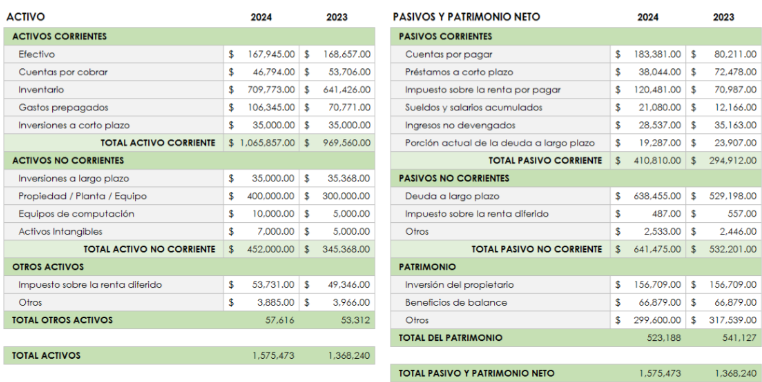
\includegraphics[width=15cm]{./assets/balance.png}
\end{center}
\begin{center}
  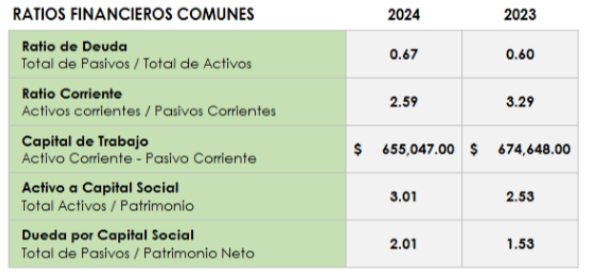
\includegraphics[width=8cm]{./assets/ratios_financieros.png}
\end{center}

\subsection{Estado de Resultados}

El estado de resultados es también conocido como estado de ganancias y pérdidas. Es un reporte financiero que muestra de manera minuciosa la situación de la empresa, es decir, si obtuvo ganancia o pérdidas en el ejercicio de un ciclo contable.

\begin{center}
  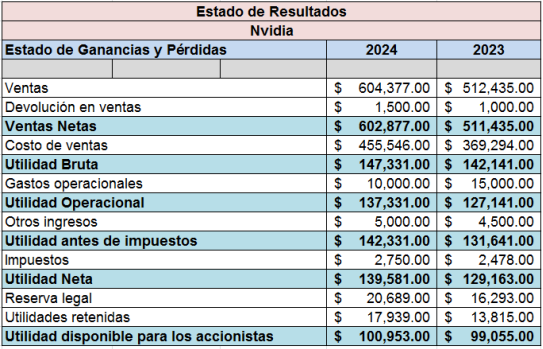
\includegraphics[width=15cm]{./assets/estado_resultados.png}
\end{center}

\newpage

\section{Indicadores de gestión financiera}

\begin{itemize}
  \item \textbf{Ratios de liquidez:} Los ratios de liquidez de Nvidia, en este caso liquidez corriente, evalúa su capacidad para cumplir con sus obligaciones a corto plazo y su solvencia financiera. Los ratios de liquidez se pueden calcular de la siguiente manera:
  
  \begin{equation}
    \text{Liquidez corriente} = \frac{\text{Activos corrientes}}{\text{Pasivos corrientes}}
\end{equation}

Para este caso y en el 2024:

\begin{equation}
    \text{Liquidez corriente} = \frac{1,065,857}{410,810} = 2.59
\end{equation}


  Se puede interpretar este resultado como que Nvidia tiene 2.59 veces más activos corrientes que pasivos corrientes, lo que indica una buena capacidad para cumplir con sus obligaciones a corto plazo.

  \item \textbf{Ratios de endeudamiento:} Los ratios de endeudamiento de Nvidia, como la razón de endeudamiento y la razón de cobertura de intereses, evalúan su nivel de endeudamiento y su capacidad para cumplir con sus obligaciones financieras. Los ratios de endeudamiento se pueden calcular de la siguiente manera:
  
  \begin{equation}
    \text{Ratio de endeudamiento} = \frac{\text{Pasivos totales}}{\text{Activos totales}}
  \end{equation}

  Para este caso y en el 2024:

  \begin{equation}
      \text{Ratio de endeudamiento} = \frac{1052285}{1575473} = 0.67
  \end{equation}

  Se puede interpretar este resultado como que el 67\% de los activos de Nvidia están financiados con deuda, lo que indica un nivel moderado de endeudamiento.

  \item \textbf{Ratios de rentabilidad:} Los ratios de rentabilidad de Nvidia, como el retorno sobre activos y el retorno sobre patrimonio, miden su capacidad para generar utilidades a partir de sus activos y patrimonio. Los ratios de rentabilidad se pueden calcular de la siguiente manera:
  
  \begin{equation}
    \text{Retorno sobre activos} = \frac{\text{Utilidad neta}}{\text{Activos totales}}
  \end{equation}

  \item \textbf{Ratios de eficiencia:} Los ratios de eficiencia de Nvidia, como la rotación de activos y la rotación de inventarios, evalúan su eficiencia en la gestión de sus activos y operaciones. Los ratios de eficiencia se pueden calcular de la siguiente manera:
  
  \begin{equation}
    \text{Rotación de activos} = \frac{\text{Ventas netas}}{\text{Activos totales}}
  \end{equation}

\end{itemize}

\newpage

\section{Cadena de valor de McKinsey}

El modelo de McKinsey mezcla las funciones internas de la empresa y la visión global del sector, definiendo el “sistema de negocio”. Para utilizar esta herramienta debemos clasificar dentro de las siguientes columnas, aquellos factores que definan la ventaja competitiva de la empresa. Aquellas que son necesarias para satisfacer al cliente, las que nos diferencian de la competencia y que más contribuyen a la formación de valor para la empresa.

A continuación, se muestra un ejemplo de la cadena de valor de McKinsey para Nvidia:

\begin{center}
  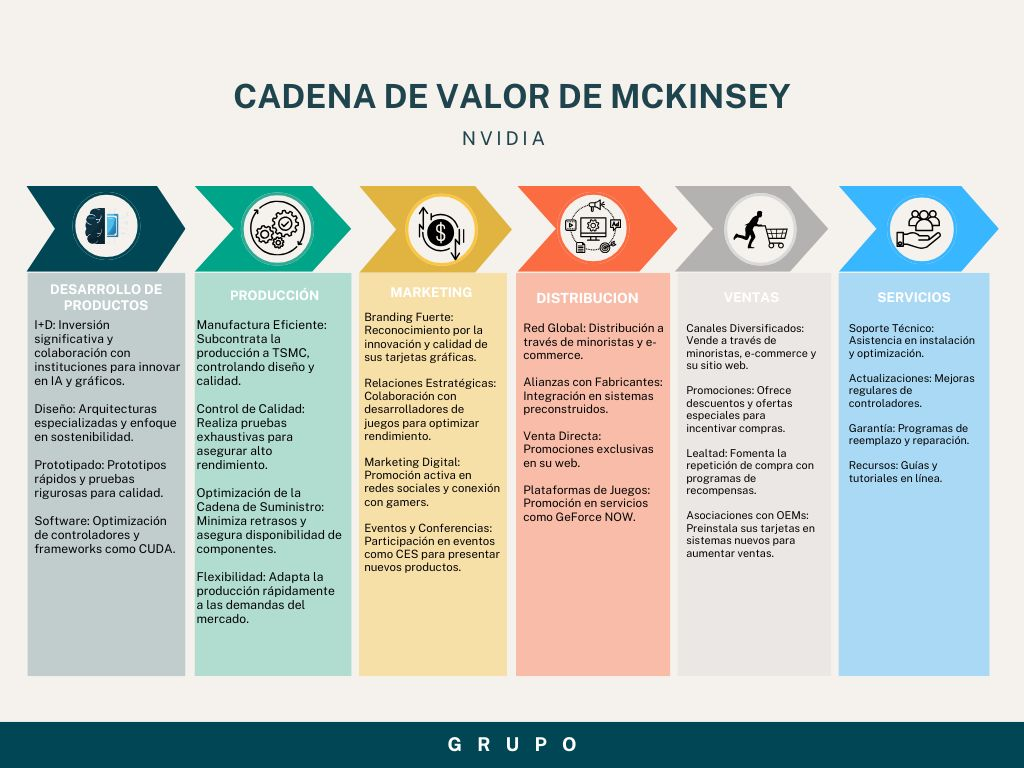
\includegraphics[width=15cm]{./assets/WhatsApp Image 2024-10-24 at 9.53.00 AM.jpeg}
\end{center}


\newpage

\section{Planificación de la gestión operativa}
\vspace{-0.5cm}
Para evaluar la planificación y monitoreo de la gestión operativa de Nvidia, en primer lugar donsideraremos la creación de un plan operativo anual o POA.
\vspace{-0.5cm}
\subsection{Plan operativo anual (POA)}
\vspace{-0.5cm}
El POA es un documento que detalla las metas y objetivos operativos de la empresa para el próximo año, así como las acciones y recursos necesarios para alcanzarlos. El POA debe estar alineado con el plan estratégico de la empresa y contener indicadores de gestión para monitorear su cumplimiento.
\vspace{-0.5cm}
\begin{enumerate}
  \item \textbf{Plan estratégico:} Necesitaremos la visión de la empresa además de las estrategias y objetivos a largo plazo.
  \begin{itemize}
    \item \textbf{Visión:} Ser líder en el mercado de tarjetas gráficas y soluciones de cómputo de alto rendimiento para el año 2026.
    \item \textbf{Estrategias:} Desarrollar nuevas GPU con mayor rendimiento y eficiencia energética, expandir la presencia en mercados emergentes y fortalecer la relación con los socios comerciales. 
  \end{itemize}
  \item \textbf{Reducción del alcance:} Se limita el desarrollo de la estrategia al área de investigación y desarrollo de nuevas GPU.
  \item \textbf{Identificaión de los participantes:} Se asignan responsabilidades a los equipos de investigación y desarrollo. Científicos, ingenieros y diseñadores.
  \item \textbf{Creación del plan operativo:} Las acciones que se llevarán a cabo incluyen la investigación de nuevas tecnologías, el diseño de prototipos y la realización de pruebas de rendimiento.
  \item \textbf{¿Cómo se medirá el éxito?:} Se utilizarán indicadores de gestión como el tiempo de desarrollo, el rendimiento de las nuevas GPU y la satisfacción del cliente.
\end{enumerate}

\begin{table}[ht]
\centering
\begin{tabularx}{\textwidth}{|X|X|X|X|X|X|} % Usar X para columnas ajustables
\hline
\textbf{Acciones} & \textbf{Fechas} & \textbf{Recursos necesarios} & \textbf{Presupuesto} & \textbf{KPI} & \textbf{Responsable} \\ \hline
Investigación de nuevas tecnologías para GPU & Enero 2024 - Junio 2024 & Equipos de laboratorio, personal técnico & $500,000$ USD & Informe de investigación completo, progreso del 70\% & Equipo de I+D \\ \hline
Diseño de prototipos de GPU de alto rendimiento & Julio 2024 - Septiembre 2024 & Ingenieros, diseñadores, software CAD & $750,000$ USD & Prototipo diseñado, pruebas iniciales completadas & Departamento de ingeniería \\ \hline
Pruebas de rendimiento y optimización de GPU & Octubre 2024 - Diciembre 2024 & Laboratorios de pruebas, testers & $300,000$ USD & GPU optimizada, rendimiento mejorado en un 15\% & Equipo de pruebas y calidad \\ \hline
Relación con socios comerciales para distribución & Noviembre 2024 - Diciembre 2024 & Equipos de ventas y marketing & $200,000$ USD & Acuerdos firmados con 3 nuevos distribuidores & Departamento de ventas y marketing \\ \hline
\end{tabularx}
\caption{Tabla del Plan Operativo Anual (POA) para el desarrollo de nuevas GPU}
\end{table}

\newpage

\section{Monitoreo de la gestión operativa}

Para monitorear la gestión operativa de Nvidia, se deben establecer indicadores clave de rendimiento (KPI) que permitan evaluar el desempeño de las operaciones y la eficiencia de los procesos. Algunos KPI relevantes para Nvidia incluyen:

\begin{enumerate}
  \item \textbf{Tiempo de desarrollo de nuevas GPU:} Mide el tiempo que se tarda en investigar, diseñar y probar nuevas GPU, desde la concepción hasta la producción.
  \item \textbf{Rendimiento de las nuevas GPU:} Mide la eficiencia y potencia de las nuevas GPU en comparación con los modelos anteriores y la competencia.
  \item \textbf{Satisfacción del cliente:} Mide la satisfacción de los clientes con las nuevas GPU, basada en la calidad, rendimiento y soporte técnico.
  \item \textbf{Costo de desarrollo de nuevas GPU:} Mide el costo total de investigación, diseño y pruebas de las nuevas GPU, en comparación con el presupuesto asignado.
  \item \textbf{Eficiencia de los procesos de producción:} Mide la eficiencia de los procesos de producción de las nuevas GPU, incluyendo la optimización de recursos y la reducción de desperdicios.
\end{enumerate}

Un ejemplo para el cálculo del tiempo de desarrollo de nuevas GPU puede denotarse por la siguiente fórmula:

\begin{equation}
  \text{Tiempo de desarrollo} = \frac{\text{Fecha de lanzamiento} - \text{Fecha de inicio}}{365}
\end{equation}

Para este ejemplo:

\begin{equation}
  \text{Tiempo de desarrollo} = \frac{2025 - 2024}{365} = 1 \text{ año}
\end{equation}

\newpage

\begin{thebibliography}{9}

  \bibitem{Altieri} 
  Altieri D., Martinez E., Perri M. (2018). Análisis e interpretación de un Balance General. Recuperado de: \url{https://www.econlink.com.ar/contenidos/ver/analisis-e-interpretacion-de-un-balance-general}

  \bibitem{Arnedo} 
  Arnedo G. (2012). La cadena de valor como nuevo eje de competitividad frente a los desafíos del mercado global. Recuperado de: \url{https://www.eumed.net/rev/cccss/20/cadena-valor.html}

  \bibitem{Ccahuay} 
  Ccahuay, Jara y Vasquez (2020). Plan de mejora en la gestión operativa para reducir costos de la empresa Shalom Empresarial S.A.C. Chiclayo. Recuperado de: \url{https://repositorio.utmachala.edu.ec/handle/48000/15307}

\end{thebibliography}

  
\end{document}